\documentclass{beamer}
\usetheme[progressbar=frametitle]{metropolis}
\setbeamercolor{progress bar}{ fg=p4, bg=p-1}
\setbeamercolor{title separator}{ fg=p4, bg=p-1 }

\definecolor{p-1}{HTML}{CCCCCC}
\definecolor{p0}{HTML}{D7DFC0}
\definecolor{p1}{HTML}{AECFA2}
\definecolor{p2}{HTML}{82BC92}
\definecolor{p3}{HTML}{5FA38E}
\definecolor{p4}{HTML}{49848B}
\definecolor{p5}{HTML}{3F5F7F}
\definecolor{p6}{HTML}{383D65}
\definecolor{p7}{HTML}{2C1E3E}


%\usepackage{previewNextNotes}
\usepackage{pgfpages}
\setbeameroption{show notes on second screen=right}
\setbeamertemplate{note page}[compressed]

\usepackage[absolute,overlay]{textpos}
%\usepackage[texcoord, grid,gridcolor=red!10,subgridcolor=green!10,gridunit=pt]{eso-pic}

%\usepackage{default}
%\usepackage[utf8]{inputenc}
\usepackage{HASstyle}
\newcommand\lr[1]{\left(#1\right)} 
\renewcommand{\vec}[1]{\mathbf{#1}}





\title{Molecular dynamics modeling of single asperity contact}
\author{Filip Henrik Larsen}
\institute{University of Oslo}
\date{\today}






\begin{document}
\begin{frame}
	\titlepage
\end{frame}
\note{Title frame}
\metroset{block=fill}

\section{Motivation}
\begin{frame}{Breakdown of continuum theory}
Mark Robbins 2005 \note{In 2005 Mark Robbins published an article }
\end{frame}
\begin{frame}{Contact problem}
	Mark Robbins 2006 \note{Mark Robbins 2006, Single asperity contact. Severe restrictions.}
\end{frame}
\begin{frame}{Friction}
	content...
\end{frame}
\begin{frame}{Goals}
\begin{itemize}
		\item Develop a molecular dynamics model \\
		\note[item]{Spherical cap and a flat substrate. 
		Material - Potential model}
		\item Compute contact force distribution \\
		\note[item]{Recognize contact forces. 
		Define contact forces as F12  (on G1 from G2).
		n\_vec of surface $\Rightarrow$ normal and shear components.
		Grid and average}
		\begin{itemize}
				\item Develop a method for computing per-atom forces\\ 
				\note[item]{\indent LAMMSP does not have GGA.}
				\item Develop a method to approximate the contact surface\\ 
				\note[item]{\indent Get n\_vec by Surface approximation}
		\end{itemize}
		
		\item Compute the coefficient of static friction \\
		\note[item]{Simulate same as Scheibert; probe on substrate - vary thickness.}
		
		\item Compare results to theory and to results of Robbins and Scheibert
		\note[item]{Support or object to Scheibert's claim. 
			\vfill
				\begin{block}{Molecular Dynamics}
					Simulation method
				\end{block}
				\vfill
				}
\end{itemize}
\end{frame}

\section{Molecular Dynamics}
\begin{frame}{Time-integration}
	The force acting on atom $i$ is assumed to be described by Newtons equation of motion.
	\begin{equation*}
	\sum_{i=1}^{N}\vec{F_i} = \sum_{i=1}^{N}-\nabla U_i({\bf r}^N)= m_i\vec{a_i}.
	\end{equation*}
	Once the acceleration is known, we update atom's velocity and position by applying time-integration. 
	\begin{align*}
	\vec{v_i}(t) &= \vec{v_i}(0) + \int_{0}^{t}\vec{a_i}(t) dt \\
	\vec{r_i}(t) &= \vec{r_i}(0) + \int_{0}^{t}\vec{v_i}(t) dt
	\end{align*}
	
	\note{$\vec{r}_0$ and $\vec{v}_0$ are known. }
\end{frame}
\begin{frame}{Velocity-Verlet}
	\begin{align*}
	\vec{v}^{n+1/2}	 &= \vec{v}^{n} +  \frac{\Delta t}{2}\vec{a}^n\\[2mm]
	\vec{r}^{n+1} &= \vec{r}^n + \Delta t \vec{v}^{n+1/2}	\\[2mm]
	\vec{a}^{n+1} &= -\nabla U(\vec{r}^{n+1})/m\\[2mm]
	\vec{v}^{n+1} &= \vec{v}^{n+1/2} + \frac{\Delta t}{2} \vec{a}^{n+1}
	\end{align*}
	\note{
		The most common scheme for time-integration in MD.
		
		Fast / Computationally cheap
		
		Preceise / Low error ($\Delta t^4$)
		
		I will not derive this, I only wish to show how simple it is.
		
		\vfill
		\begin{block}{Potentail}
			In order to obtain {\color[rgb]{0.8,0,0}realistic dynamics}, the potential model must {\color[rgb]{0.8,0,0}describe forces accurately}. There are many types of potentails. Many of them are material spesific. The simplest, but still commonly used potential is the {\color[rgb]{0.8,0,0} LJ potential}.
		\end{block} 		
		\vfill
	}
\end{frame}
\begin{frame}[t]{Potentials}
	\only<1-2>{\large Lennard-Jones}
	
	
	 \only<1-2>{
	 	\begin{equation*}V(r) =4\epsilon\left[\lr{\frac{\sigma}{r}}^{12} -  \lr{\frac{\sigma}{r}}^6 \right]
		\end{equation*}
	}

	\only<2>{
		\begin{figure}[H]
			\centering{
				\def\svgwidth{0.8\linewidth}
				% arara: pdflatex
\documentclass{standalone}
\usepackage{pgfplots}
\usepackage{tikz}
% set the arrows as stealth fighters
\tikzset{>=stealth}
\begin{document}
	\begin{tikzpicture}
	\begin{axis}[
	xmin=0,xmax=3.2,
	ymin=-1,ymax=1.2,
	axis lines=center,
	axis line style=->]
	\addplot[-] expression[domain=0.95:3, samples=100]{4*((1/x)^12 - (1/x)^6)};
	\draw (1.1224, -0.5) node[anchor=east] {hei};
	\end{axis}
	\end{tikzpicture}
\end{document}
			}
		\end{figure}
	}
\end{frame}
\begin{frame}[t]{Potentials}
	\only<1->{
	{\large Vashishta}\\*
	\begin{equation*}
		V(r) = \sum_{i<j} V_{ij}^{(2)}(r_{ij}) + \sum_{i<j<k} V_{ijk}^{(3)}(\vec{r}_{ij}, \vec{r}_{ik}) 
	\end{equation*}
	\\[5mm]
	}
	\only<2->{
	\begin{equation*}
			V_{ij}^{(2)}(r) = 
		\frac{H_{ij}}{\displaystyle r^{\eta_{ij}}} +
		\frac{Z_iZ_j}{r}e^{-r/r_{1s}} -
		\frac{D_{ij}}{2r^4}e^{-r/r_{4s}} - 
		\frac{W_{ij}}{r^6}
	\end{equation*}
	\\
}
	\only<3->{
	\begin{equation*}
			\hspace{-8mm}
			V_{ijk}^{(3)}(\vec{r}_{ij}, \vec{r}_{ik}) = 
			B_{ijk} \exp\lr{\frac{\xi}{r_{ij}-r_0} + \frac{\xi}{r_{ik}-r_0}}
			\frac{\lr{\cos \theta_{ijk} - \cos \theta_0}^2}{1 + C_{ijk}\lr{\cos \theta_{ijk} - \cos \theta_0}^2}
	\end{equation*} 
} 

	\note<2>{
		\begin{table}
		\begin{tabular}{lll}
			$H_{ij}$ &:& Strength of the steric repulsion \\
			$\eta_{ij}$ &:& Exponent of the steric repulsion\\
			$Z_i$ &:& Effective charge of atom $i$\\
			$r_{1s}$ &:& Screening lengths for the coulomb interaction\\
			$r_{4s}$ &:& Screening lengths for the dipole interaction\\
			$D_{ij}$ &:& Strength of the dipole interaction\\
			$W_{ij}$ &:& Strength of the Van der Waal interaction
		\end{tabular}
		\end{table}
	}
	
	\note<3>{
		\begin{table}
			\begin{tabular}{lll}
				$B_{ijk}$ &:& Strength of the three-body term \\
				$\xi$ &:& Constant parameter\\
				$C_{ijk}$ &:& Constant parameter\\
				$r$ &:& Cut-off length\\
				$\theta_{ijk}$ &:& Angle between $\vec{r}_{ji}$ and $\vec{r}_{jk}$\\
				$\theta_{0}$ &:& Equilibrium bond angle
			\end{tabular}
		\end{table}
		\vfill 
		\begin{block}{Boundary conditions}
			The potential govern the force interaction between atoms. However {\color[rgb]{0.8,0,0} which atoms} interact is decided using a {\color[rgb]{0.8,0,0} cut-off} range, and dependent on the {\color[rgb]{0.8,0,0} boundary conditions} we use.
		\end{block}
		 
		\vfill
	}
\end{frame}
\begin{frame}{Boundary conditions}
	\only<1>{
		No boundary conditions
		\vfill
		\begin{figure}
			\includegraphics[width=0.5\linewidth]{figures/BoundaryConditions/no.pdf} 
		\end{figure}
	}
	
	
	\only<2>{
		Reflecting boundary conditions
		\vfill
		\begin{figure}
			\includegraphics[width=0.5\linewidth]{figures/BoundaryConditions/reflecting.pdf} 
		\end{figure}
	}
	
	\only<3>{
		Periodic boundary conditions
		\vfill
		\begin{figure}
			\includegraphics[width=0.5\linewidth]{figures/BoundaryConditions/periodic.pdf} 
		\end{figure}
	}
	
	\note{
		\begin{itemize}
			\item Also affect atom trajectories\\
			\only<3>{\item Periodic minimum image convention}
			
		\end{itemize}
		}
\end{frame}
\begin{frame}{Measuring physical quantities}
	\only<1>{
		{\large Energy}
		\vfill
		As we assume Newtonian motion, the kinetic energy is computed simply as 
		\begin{equation*}
			E_K = \frac{1}{2}\sum_{i=1}^{N} m_i {\vec{v}_i}^2,
		\end{equation*} 
		while the potential energy is computed directly from the potential
		\begin{equation*}
			E_P = \sum_{i=1}^{N}\sum_{j>i}^{N}U(\vec{r}_i, \vec{r}_j).
		\end{equation*} 
	}
\end{frame}
\begin{frame}{Measuring physical quantities}
	\only<1>{
		{\large Temperature}
		\vfill
		For a system consisting of $N$ atoms with $f$ kinetic degrees of freedom and temperature $T$, thermodynamics state that
		\begin{equation*}
			E_k = \frac{f}{2} Nk_bT. 	\note{
				$k_b$ is the Boltzmann constant. 
				
				Since we assume point particles, we take only the translational degrees of freedom into account and ignore the rotational degrees of freedom.}
		\end{equation*}
		
		Thus we have two relations for the kinetic energy. 
		By equating these we find the instantaneous temperature given as
		\begin{equation*}\label{eq:MDtemperature}
		T = \frac{\langle m_i \vec{v_i}^2\rangle}{f\hspace{0.2mm}k_b}.
		\end{equation*}
		\note{
			
		Thus, we can approximate the instantaneous temperature using the atoms velocities.
		
		This value will fluctuate about the real value, so time-averaging is often used when measuring.
		
		In many cases it is desirable to control the temperature of the system, e.g. when using the canonical ensemble (NVT).
		Methods for doing this are called \textit{thermostats}, and are described in section 
		}
	}
\end{frame}
%\begin{frame}{Measuring physical quantities}
%	\only<3>{
%		{\large Pressure}
%		\vfill
%		
%		\note{There are many methods for computing the pressure of the system.\\}
%		Normally, for a N-body system of volume $V$ and particle density $\rho=N/V$ in the canonical ensemble, it is taken from the virial equation for pressure. 
%		\begin{equation*}
%		P = \rho k_B T + \frac{1}{dV}\Big< \sum_{i<j} \vec{F}_{ij} \cdot \vec{r}_{ij}\Big> ,
%		\end{equation*}
%		The equation is dependent on the ensemble in use.
%		\note{
%					\begin{table}
%						\begin{tabular}{lll}
%							$d$ &:& Number of dimensions \\
%							$\vec{F}_{ij}$ &:& Force contribution on atom $i$ from atom $j$
%						\end{tabular}
%					\end{table}
%					
%		This expression assume constant $NVT$, i.e. the canonical ensemble.
%		
%		The equation will not be the same for the micro-canonical ensemble.	
%		}
%		
%		}	
%\end{frame}


\begin{frame}{Thermostats}
	Thermostats are alterations implemented to control the average temperature. \\[5mm]
	
	Common thermostats:
	\begin{itemize}
		\item \only<2>{{\bf Berendsen}} \only<1,3->{Berendsen}
		\item \only<3>{{\bf Andersen}} \only<1,2,4>{Andersen}
		\item  \only<4>{{\bf Nosé-Hoover}} \only<-3>{Nosé-Hoover}
	\end{itemize}
	\note{
		%We are necesserily required to control the temperature in order to simulate the canonical ensemble ($NVT$).
		\begin{description}
			\item[Berendsen]
			Rescales velocities so that the temperature approaches that of the heat bath.
			How fast the velocities should converge to that of the heat bath, can be tuned.
			
			\item[Andersen]
			Assigns a randomly chosen atom a randomly distributed velocity with the target temperature as average.
			
			\item[Nosé-Hoover]
			Incorporates a fictitious frictional force in the equation of motion. 
		\end{description}
		
		Berendsen and Andersen does not produce realistic dynamics due to the direct scaling of the temperature. Andersen also disturbes lattice vibrations and decorrelates the system, rendering it unfit when measuring diffusion coefficient.
		
		The Nosé-Hoover thermostat is the {\color{red}most commonly} used thermostat, because it produces accurate dynamics.
		}
\end{frame}

\section{LAMMPS}
\begin{frame}{About LAMMPS}
	\phantom{i}{\color{p4} L}arge-scale {\color{p4}A}tomic/{\color{p4}M}olecular {\color{p4}M}assively {\color{p4}P}arallel {\color{p4}S}imulator
	\vfill
	A classical molecular dynamics simulation code designed to run efficiently on parallel computers. 
	
	Development began in the mid 1990s, and is still ongoing.
	
	Open-source
	
	Extensive and user friendly documentation.
	
	\note{Show examples with Atomify!
		\begin{block}{Simulations}
			We will precent:
			\begin{itemize}
				\item How our simulations were set up\\
				\item The most important details of the simulations \\
				\item Lastly, we will post and discuss the results
			\end{itemize}
		\end{block}}
\end{frame}

\section{Simulations}
\begin{frame}{Preparing a simulation}
	We need to consider the following aspects of the simulation:
	\begin{itemize}
		\item Geometry of the system
		\item Boundary conditions
		\item Material
		\item Potential model
		\item Ensemble
		\item Other restrictions
		\item Applied actions
	\end{itemize}
	\note{\vfill
		\begin{block}{Creating a crystal}
			Place atoms into inital positions.\\
			Unit cell of $\beta$-cristobalite
		\end{block}
		\vfill
		}
	
\end{frame}
\begin{frame}{Creating a crystal}
	
\only<1>{
	\vspace{-3mm}
	\lstinputlisting[language=LammpsData, basicstyle=\fontsize{5.5pt}{6.5pt}\selectfont, firstline=3, linewidth=1.1\linewidth]{../SiO2/large/beta-cristobalite.lt}
	}

\only<2>{
	\begin{figure}
		\includegraphics[width=0.5\linewidth]{figures/CreatingSystem/buildingBlocks/frame000.png}
	\end{figure}
}
\only<3>{
	\begin{figure}
		\includegraphics[width=0.5\linewidth]{figures/CreatingSystem/buildingBlocks/frame001.png}
	\end{figure}
}
\only<4>{
	\begin{figure}
		\includegraphics[width=0.5\linewidth]{figures/CreatingSystem/buildingBlocks/frame002.png}
	\end{figure}
}
\only<5>{
	\begin{figure}
		\includegraphics[width=0.5\linewidth]{figures/CreatingSystem/buildingBlocks/frame003.png}
	\end{figure}
}
\only<6>{
	\begin{figure}
		\includegraphics[width=0.5\linewidth]{figures/CreatingSystem/buildingBlocks/frame004.png}
	\end{figure}
}
\only<7>{
	\begin{figure}
		\includegraphics[width=0.5\linewidth]{figures/CreatingSystem/buildingBlocks/frame005.png}
	\end{figure}
}
\only<8>{
	\begin{figure}
		\includegraphics[width=0.5\linewidth]{figures/CreatingSystem/buildingBlocks/frame006.png}
	\end{figure}
}
\only<9>{
	\begin{figure}
		\includegraphics[width=0.5\linewidth]{figures/CreatingSystem/buildingBlocks/frame007.png}
	\end{figure}
}
\only<10>{
	\begin{figure}
		\includegraphics[width=0.5\linewidth]{figures/CreatingSystem/buildingBlocks/frame008.png}
	\end{figure}
}
\only<11>{
	\begin{figure}
		\includegraphics[width=0.5\linewidth]{figures/CreatingSystem/buildingBlocks/frame009.png}
	\end{figure}
}
\only<12>{
	\begin{figure}
		\includegraphics[width=0.5\linewidth]{figures/CreatingSystem/buildingBlocks/frame010.png}
	\end{figure}
}
\only<13>{
	\begin{figure}
		\includegraphics[width=0.5\linewidth]{figures/CreatingSystem/buildingBlocks/frame011.png}
	\end{figure}
}
\only<14>{
	\begin{figure}
		\includegraphics[width=0.5\linewidth]{figures/CreatingSystem/buildingBlocks/frame012.png}
	\end{figure}
}
\only<15>{
	\begin{figure}
		\includegraphics[width=0.5\linewidth]{figures/CreatingSystem/buildingBlocks/frame013.png}
	\end{figure}
}
\only<16>{
	\begin{figure}
		\includegraphics[width=0.5\linewidth]{figures/CreatingSystem/buildingBlocks/frame014.png}
	\end{figure}
}
\only<17>{
	\begin{figure}
		\includegraphics[width=0.5\linewidth]{figures/CreatingSystem/buildingBlocks/frame015.png}
	\end{figure}
}
\only<18>{
	\begin{figure}
		\includegraphics[width=0.5\linewidth]{figures/CreatingSystem/buildingBlocks/frame016.png}
	\end{figure}
}
\only<19>{
	\begin{figure}
		\includegraphics[width=0.5\linewidth]{figures/CreatingSystem/buildingBlocks/frame017.png}
	\end{figure}
}
\only<20>{
	\begin{figure}
		\includegraphics[width=0.5\linewidth]{figures/CreatingSystem/buildingBlocks/frame018.png}
	\end{figure}
}
\only<21>{
	\begin{figure}
		\includegraphics[width=0.5\linewidth]{figures/CreatingSystem/buildingBlocks/frame019.png}
	\end{figure}
}
\only<22>{
	\begin{figure}
		\includegraphics[width=0.5\linewidth]{figures/CreatingSystem/buildingBlocks/frame020.png}
	\end{figure}
}
\only<23>{
	\begin{figure}
		\includegraphics[width=0.5\linewidth]{figures/CreatingSystem/buildingBlocks/frame021.png}
	\end{figure}
}
\only<24>{
	\begin{figure}
		\includegraphics[width=0.5\linewidth]{figures/CreatingSystem/buildingBlocks/frame022.png}
	\end{figure}
}
\only<25>{
	\begin{figure}
		\includegraphics[width=0.5\linewidth]{figures/CreatingSystem/buildingBlocks/frame023.png}
	\end{figure}
}
\only<26>{
	\begin{figure}
		\includegraphics[width=0.5\linewidth]{figures/CreatingSystem/buildingBlocks/frame024.png}
	\end{figure}
}
\only<27>{
	\begin{figure}
		\includegraphics[width=0.5\linewidth]{figures/CreatingSystem/buildingBlocks/frame025.png}
	\end{figure}
}
\only<28>{
	\begin{figure}
		\includegraphics[width=0.5\linewidth]{figures/CreatingSystem/buildingBlocks/frame026.png}
	\end{figure}
	\note<28>{\begin{block}{$15^3$-Cube}
			We make a large cube...
		\end{block}}
}
\only<29>{
	\vspace{2mm}
	\begin{figure}
		\includegraphics[width=0.7\linewidth]{figures/CreatingSystem/cube.png}
	\end{figure}
		\note<29>{
			Density: 2.2114 g/cm$^3$
			\vfill
			\begin{block}{Melting point}
			    Check basic properties of the system:
				
				Density
				
				Melting point
			\end{block}
			\vfill
			}
}
\end{frame}



\begin{frame}{Melting point}
	\only<1>{
	\begin{equation*}
	D = \frac{\langle r^2(t)\rangle}{2dt},
	\end{equation*}
	\begin{equation*}
	\langle r^2(t)\rangle = \frac{1}{N}\sum_{i=1}^{N}\lr{\vec{r}_i(t)-\vec{r}_i(0)}^2
	\end{equation*}
	\vfill
}

\only<2>{
	\begin{figure}[H]
		\includegraphics[width=0.7\linewidth]{../SiO2/msd/figures/msdplot_01500.pdf}
	\end{figure}
}
\only<3>{
	\begin{figure}[H]
		\includegraphics[width=0.7\linewidth]{../SiO2/msd/figures/msdplot_01550.pdf}
	\end{figure}
}
\only<4>{
	\begin{figure}[H]
		\includegraphics[width=0.7\linewidth]{../SiO2/msd/figures/msdplot_01600.pdf}
	\end{figure}
}
\only<5>{
	\begin{figure}[H]
		\includegraphics[width=0.7\linewidth]{../SiO2/msd/figures/msdplot_01650.pdf}
	\end{figure}
}
\only<6>{
	\begin{figure}[H]
		\includegraphics[width=0.7\linewidth]{../SiO2/msd/figures/msdplot_01700.pdf}
	\end{figure}
}
\only<7>{
	\begin{figure}[H]
		\includegraphics[width=0.7\linewidth]{../SiO2/msd/figures/msdplot_01750.pdf}
	\end{figure}
}
\only<8>{
	\begin{figure}[H]
		\includegraphics[width=0.7\linewidth]{../SiO2/msd/figures/msdplot_01800.pdf}
	\end{figure}
}
\only<9>{
	\begin{figure}[H]
		\includegraphics[width=0.7\linewidth]{../SiO2/msd/figures/msdplot_01850.pdf}
	\end{figure}
}
\only<10>{
	\begin{figure}[H]
		\includegraphics[width=0.7\linewidth]{../SiO2/msd/figures/msdplot_01900.pdf}
	\end{figure}
}
\only<11>{
	\begin{figure}[H]
		\includegraphics[width=0.7\linewidth]{../SiO2/msd/figures/msdplot_01950.pdf}
	\end{figure}
}
\only<12>{
	\begin{figure}[H]
		\includegraphics[width=0.7\linewidth]{../SiO2/msd/figures/msdplot_02000.pdf}
	\end{figure}
}
	\only<13>{
		\begin{figure}[H]
			\includegraphics[width=0.7\linewidth]{../SiO2/msd/figures/msdTransparent.pdf}
		\end{figure}
		}
\note<1>{
	\begin{table}
		\begin{tabular}{lll}
			$D$ &:& Self diffusion coefficient \\
			$d$ &:& Number of dimension \\
			$t$ &:& Time\\
			$\langle r^2(t)\rangle$ &:& Mean square displacement\\
			$r$ &:& Position\\
			$N$ &:& Number of atoms
		\end{tabular}
	\end{table}
}
\note<13>{1986K - Wikipedia
	
	Deviations less than $20\%$ from the experimental results is considered a pass, as stated by the developers of the potential. 
	
	Some qualitative detail that is lost. We should focus on quantitative behavior. 
	}

\end{frame}

\section{Numerical simulations}
\note{
	\begin{block}{Shaping the system}
		We carve out regions to obtain the desired geometry.
	\end{block}
	}



\begin{frame}{Configuring the  simulation}
	\only<1>{
	\begin{figure}
		\includegraphics[width=0.9\linewidth]{figures/hysteresis/animation/hysteresis3.png}
	\end{figure}
}
	\only<2>{
		\begin{figure}
			\includegraphics[width=0.9\linewidth]{figures/hysteresis/animation/hysteresis6.png}
		\end{figure}
	}
	\only<3>{
		\begin{figure}
			\includegraphics[width=0.9\linewidth]{figures/hysteresis/animation/hysteresis9.png}
		\end{figure}
	}
		\only<4>{
			\begin{figure}
				\includegraphics[width=0.9\linewidth]{figures/hysteresis/animation/hysteresis12.png}
			\end{figure}
		}
	\only<5>{
		\begin{figure}
			\includegraphics[width=0.9\linewidth]{figures/hysteresis/animation/hysteresis15.png}
		\end{figure}
	}
	\note{
		Regions, groups, delete, fix nvt
		
		Used in both experiments (but with varying thickness in problem 2).
		
		Frozen regions (top/bottom).
		
		Lowering sphere $\Rightarrow$ $\dfrac{\partial v}{\partial t} = 0$ or $\dfrac{\partial F}{\partial t} = 0$.
\begin{enumerate}
	\item Lower sphere with constant velocity $\rightarrow$ Hold at constant height $\rightarrow$ Compute force distribution 
	\item Lower sphere by linearly increasing load $\rightarrow$ Keep load constant $\rightarrow$ Apply shear force
\end{enumerate}
		}
\end{frame}


\begin{frame}[t]{Computing contact force distribution}
	Contact forces acts between two bodies at the area of contact. 
	
	They can be decomposed into normal and shear forces.
	
	Challenging to compute in MD because:
	\begin{itemize}
		\item[-] The contact surface has to be defined.
		\item[-] We must distinguish between contact and non-contact forces.
	\end{itemize}
	
	\note{
		Contact can be defined as the maximum distance one experiences repulsive net-force on the surface atoms.
		}
\end{frame}


\begin{frame}[t]{Custom compute}
	Stores the net force acting on each atom of one group, from all atoms of the other group.
	
	Per-atom version of \texttt{compute group/group}.
	
	Verified by using Lennard-Jones and few particles. 
	
	Integrated with the LAMMPS distribution.
	
	Must rebuild LAMMPS with special sequence of commands. 
\end{frame}

{\setbeamercolor{background canvas}{bg=white}
\begin{frame}{Distribution of magnitude of contact force}
	\centering
	\begin{figure}
			\includegraphics[width=0.8\linewidth,  trim={15mm 2mm 7mm 2mm}, clip]{figures/forceDistribution/forces/absoluteForceDistribution.pdf}
	\end{figure}
\end{frame}
}

{\setbeamercolor{background canvas}{bg=white}
	\begin{frame}{Distribution of z-component of contact force}
		\centering
		\begin{figure}
			\includegraphics[width=0.8\linewidth,  trim={15mm 2mm 7mm 2mm}, clip]{figures/forceDistribution/forces/zForceDistribution.pdf}
		\end{figure}
	\end{frame}
}




\setbeamercolor{background canvas}{bg=white}
\begin{frame}{Defining the surface}
\only<1>{
Define <<surface atoms>> of one group.

Partition the system into a 2D grid (in the xy-plane).

Apply least squares plane regression on the <<surface atoms>> in each element of the grid.
\\[1cm]
Equation to solve:
\begin{equation*}
z = ax + by + c
\end{equation*}
Yields normal vector:
\begin{equation*}
\vec{n} = [a,b,1]
\end{equation*}
}
\end{frame}


\begin{frame}{Defining the surface}
\begin{figure}
\includegraphics[width=1\linewidth, trim={30mm 47mm 22mm 48mm}, clip]{figures/forceDistribution/surface/approximation23_5.pdf}
\end{figure}
\end{frame}



\begin{frame}{Contact force distribution}
	\begin{figure}[H]
		\centering
		\includegraphics[width=\linewidth, trim={8mm 42mm 12mm 17mm}, clip]{figures/forceDistribution/radialResults/ALL_timestep_110000.pdf}
	\end{figure}
		\note{Spatial and radial distribution of the magnitude of force, as well as normal and shear force. 
			The spatial distributions shown on the top row are equivalent to the ones in figure \ref{fig:forceDistributions}, only in polar coordinates. 
			The magnitude of the force components (y-axis) represents the force acting on a square of area $7.12\mathring{A}\times7.12\mathring{A}$.
			The values at given radii $r$ in the bottom figures, are the average value of a column at that $r$ in the top row.
			The units of $r$ is unit cell length (7.12$\mathring{A}$).
			This is an average distribution from 10 simulations. 
			The shaded areas in the radial distribution represents the standard deviation.
			In the simulations we pushed a sphere with radius of curvature $R=200\mathring{A}$,  40$\mathring{A}$ into a half-space of size $327.52\mathring{A} \times 327.52\mathring{A} \times 157.64 \mathring{A}$. 
		}
\end{frame}



\section{Results - 1}


\begin{frame}{Results}
	\centering
\only<1>{
	h = $-5\mathring{A}$
	\begin{figure}[H]
		\includegraphics[width=\linewidth, trim={8mm 0mm 35mm 3}, clip]{figures/forceDistribution/radialResults/timestep_065000.pdf}
	\end{figure}
}
\only<2>{
	h = $0\mathring{A}$
	\begin{figure}[H]
		\includegraphics[width=\linewidth, trim={8mm 0mm 35mm 3}, clip]{figures/forceDistribution/radialResults/timestep_070000.pdf}
	\end{figure}
}
\only<3>{
	h = $5\mathring{A}$
	\begin{figure}[H]
		\includegraphics[width=\linewidth, trim={8mm 0mm 35mm 3}, clip]{figures/forceDistribution/radialResults/timestep_075000.pdf}
	\end{figure}
}
\only<4>{
	h = $10\mathring{A}$
	\begin{figure}[H]
		\includegraphics[width=\linewidth, trim={8mm 0mm 35mm 3}, clip]{figures/forceDistribution/radialResults/timestep_080000.pdf}
	\end{figure}
}
\only<5>{
	h = $15\mathring{A}$
	\begin{figure}[H]
		\includegraphics[width=\linewidth, trim={8mm 0mm 35mm 3}, clip]{figures/forceDistribution/radialResults/timestep_085000.pdf}
	\end{figure}
}
\only<6>{
	h = $20\mathring{A}$
	\begin{figure}[H]
		\includegraphics[width=\linewidth, trim={8mm 0mm 35mm 3}, clip]{figures/forceDistribution/radialResults/timestep_090000.pdf}
	\end{figure}
}
\only<7>{
	h = $25\mathring{A}$
	\begin{figure}[H]
		\includegraphics[width=\linewidth, trim={8mm 0mm 35mm 3}, clip]{figures/forceDistribution/radialResults/timestep_095000.pdf}
	\end{figure}
}
\only<8>{
	h = $30\mathring{A}$
	\begin{figure}[H]
		\includegraphics[width=\linewidth, trim={8mm 0mm 35mm 3}, clip]{figures/forceDistribution/radialResults/timestep_100000.pdf}
	\end{figure}
}
\only<9>{
	h = $35\mathring{A}$
	\begin{figure}[H]
		\includegraphics[width=\linewidth, trim={8mm 0mm 35mm 3}, clip]{figures/forceDistribution/radialResults/timestep_105000.pdf}
	\end{figure}
}
\only<10>{
	h = $40\mathring{A}$
	\begin{figure}[H]
		\includegraphics[width=\linewidth, trim={8mm 0mm 35mm 3}, clip]{figures/forceDistribution/radialResults/timestep_110000.pdf}
	\end{figure}
}
\end{frame}

























\end{document}


